\documentclass[11pt]{article}
\usepackage[margin=1in]{geometry}
\usepackage[T1]{fontenc}
\usepackage{lmodern}
\usepackage{microtype}
\usepackage{amsmath,amssymb}
\usepackage{booktabs,tabularx,array}
\usepackage{enumitem}
\usepackage{xcolor}
\usepackage{graphicx}
\usepackage[section]{placeins}
\usepackage{listings}
\usepackage{tikz}
\usetikzlibrary{arrows.meta,positioning}
\usepackage[obeyspaces,spaces]{url}
\usepackage[hidelinks]{hyperref}

\setlist{itemsep=2pt,topsep=4pt}
\setlength{\parskip}{5pt}
\setlength{\parindent}{0pt}
\setlength{\emergencystretch}{3em}
\renewcommand{\arraystretch}{1.25}
\newcolumntype{Y}{>{\raggedright\arraybackslash}X}

\definecolor{codebg}{RGB}{247,247,250}
\definecolor{codeframe}{RGB}{200,200,210}
\definecolor{keyword}{RGB}{30,60,140}
\definecolor{comment}{RGB}{100,110,120}
\definecolor{string}{RGB}{150,60,20}
\definecolor{notebg}{RGB}{238,244,252}
\definecolor{okbg}{RGB}{232,246,234}
\definecolor{warnbg}{RGB}{253,240,232}
\definecolor{linkc}{RGB}{20,80,170}
\definecolor{enumc}{RGB}{42,120,214}
\definecolor{sampc}{RGB}{235,104,52}
\hypersetup{colorlinks=true,linkcolor=linkc,urlcolor=linkc,filecolor=linkc}

\lstdefinestyle{java}{language=Java, basicstyle=\ttfamily\small, columns=fullflexible, keepspaces=true,
  keywordstyle=\color{keyword}\bfseries, commentstyle=\color{comment}\itshape, stringstyle=\color{string},
  backgroundcolor=\color{codebg}, frame=single, rulecolor=\color{codeframe}, breaklines=true,
  showstringspaces=false, xleftmargin=4pt, xrightmargin=4pt, aboveskip=6pt, belowskip=6pt}
\lstset{style=java}

\newcommand{\code}[1]{\texttt{#1}}
\newcommand{\shadedbox}[3]{\par\smallskip\noindent\colorbox{#1}{\parbox{\dimexpr\linewidth-2\fboxsep}{\textbf{#2}\par #3}}\par\smallskip}
\newcommand{\takeaway}[1]{\shadedbox{okbg}{In short}{#1}}
\newcommand{\note}[1]{\shadedbox{notebg}{Note}{#1}}
\newcommand{\caveat}[1]{\shadedbox{warnbg}{Caveat}{#1}}
\newcommand{\docsdir}{../}
\def\thisdoc{hybrid}
% Shared cross-document links for the ParaDEVS documents. Each document defines \docsdir (path from its folder to
% docs/) and \thisdoc (its key below), then \input's this file.
%
% \doclink{path relative to docs/}{text}: a link to another PDF. Links are plain URI actions (file:///...), because
% Edge, Chrome and VS Code's PDF viewers ignore hyperref's usual "open another PDF" (GoToR) links. The absolute
% address comes from docroot.tex, which scripts/build_docs.sh regenerates; rerun it if the folder moves.
%
% \relateddocs: the "ParaDEVS documents" box listing every document, with the current one marked.
\InputIfFileExists{\docsdir docroot.tex}{}{\gdef\docroot{.}}
\providecommand{\thisdoc}{}
\definecolor{pdlink}{RGB}{20,80,170}
\definecolor{pdrelbg}{RGB}{243,246,252}
\definecolor{pdrelframe}{RGB}{190,200,220}
\makeatletter
\newcommand{\doclink}[2]{\hyper@linkurl{\textcolor{pdlink}{\textbf{#2}}}{\docroot/#1}}
\newcommand{\pd@item}[4]{% key, path, title, description
  \def\pd@key{#1}%
  \item \ifx\pd@key\thisdoc\textbf{#3} (this document)\else\doclink{#2}{#3}\fi: #4}
\newcommand{\relateddocs}{\par\medskip\noindent
  \fcolorbox{pdrelframe}{pdrelbg}{\parbox{\dimexpr\linewidth-2\fboxsep-2\fboxrule}{\small
  \textbf{ParaDEVS documents.} The entry point is \doclink{ParaDEVS_Start_Here.pdf}{Start Here}, a reading guide
  that links every document.
  \begin{itemize}[leftmargin=1.4em,itemsep=0pt,topsep=2pt]
  \pd@item{report}{report/ParaDEVS_Build_Report.pdf}{Build Report}{what has been built, how it was verified, what is next}
  \pd@item{howto}{howto/ParaDEVS_HowTo.pdf}{How-To Guide}{setup, tutorials, API reference, troubleshooting}
  \pd@item{architecture}{architecture/ParaDEVS_Architecture.pdf}{Architecture Guide}{how the library works and how to read results}
  \pd@item{rl}{rl/ParaDEVS_RL_Plan.pdf}{RL Plan}{reinforcement-learning plan, analysis and results}
  \pd@item{control}{rl/ParaDEVS_Control_Spec.pdf}{Control Spec}{action selection: Para.decide, graph-mode planning, value and policy iteration}
  \pd@item{hybrid}{rl/ParaDEVS_Hybrid_Study.pdf}{Hybrid Study}{which draws to enumerate or sample, and how cost grows with lookahead}
  \pd@item{fastcopy}{engine/ParaDEVS_FastCopy_Proposal.pdf}{Fast-Copy Proposal}{why the engine replays steps, where time goes, how to speed it up}
  \end{itemize}}}\par\medskip}
\makeatother

\graphicspath{{../../rl/experiments/results/}}

\title{\textbf{ParaDEVS Library}\\[4pt]\large Hybrid selection and cost growth: when to enumerate a draw, when to
sample it, and when exact expansion is cheaper}
\author{ParaDEVS Library workspace, Binghamton}
\date{October 16, 2026}

\begin{document}
\maketitle

\begin{center}
\begin{minipage}{0.88\linewidth}\small
\textbf{How to read this report.} Section~\ref{sec:glance} is a one-page summary; if you read nothing else, read
that. Every later section opens with a green ``In short'' box, so you can skim by reading only those boxes. Terms are
defined in the glossary (Appendix~\ref{app:glossary}). The study extends the variance analysis of the
\doclink{rl/ParaDEVS_RL_Plan.pdf}{RL Plan} (Section ``Monte Carlo at every stage, plus merging: variance''); the
engine itself is described in the \doclink{report/ParaDEVS_Build_Report.pdf}{Build Report}.
\end{minipage}
\end{center}

\relateddocs

\tableofcontents
\newpage

%=====================================================================
\section{At a glance}\label{sec:glance}

{\small
\renewcommand{\arraystretch}{1.12}
\begin{tabularx}{\linewidth}{@{}>{\bfseries\raggedright\arraybackslash}p{2.5cm}Y@{}}
\toprule
Question & When a model makes several random draws per step, which draws should the engine follow
  exhaustively and which should it sample? And as the lookahead $n$ grows, when is exact expansion cheaper than
  any sampler?\\
Test bed & Slippery FrozenLake 8$\times$8 (two draws per step: the policy's \emph{action}, 4 outcomes, and the
  ice's \emph{slip}, 3 outcomes) and the 19-state random walk. $n$-step expected targets with $V=V^\pi$, so the
  exact answer is known. $\varepsilon$-soft optimal policy, $\varepsilon=0.2$, $\gamma=0.99$.\\
Which hybrid wins & \textbf{Sample the action, enumerate the slip, merge}, best with budget allocation for the
  action. Its variance$\times$work is the lowest of all sampled configurations at every $n$ and $k$: $1.3$--$2.9\times$
  better than the best one-draw sampler and $2.3$--$6.7\times$ better than plain rollouts. The reverse (enumerate the
  action, sample the slip) is the \emph{worst} merged configuration, $5$--$8\times$ worse than the winner at equal
  sampling.\\
Why & The law of total variance splits a rollout's variance into a policy part and a slip part. The slip carries
  \textbf{88\%} of it (77--95\% across start states and $n$), the policy only 12\%. Enumerating the slip removes
  most of the noise for a branching of only 3.\\
Unbiased & Every sampled mean is within 3.2 standard errors of the exact value, over about 1{,}200 (configuration,
  start state) cells, and a new 12-check test (\code{VerifyHybrid}) confirms the hybrids are unbiased.\\
Cost growth & Without merging, exact work grows like $b^n$: $66{,}232$ departures at $n=8$ on FrozenLake, over
  the 50k live-branch cap from $n=9$. With safe merging it grows polynomially and then \textbf{linearly}, once the
  set of live states is full: from $n\approx11$ on FrozenLake (53 states) and $n\approx14$ on the random walk.\\
A finding & The merge key contains the observation, and \code{MdpWalker}'s observation lags the state by one step,
  so branches merge on (previous state, state) pairs. A lag-free observation (\code{LagFreeWalker}) merges on the
  state alone and cuts exact work by up to $2.8\times$ (FrozenLake, $n=12$: 4{,}609 $\to$ 1{,}642; random walk
  $1.7\times$). Both are predicted \emph{exactly} by a level-by-level count of reachable states.\\
Crossover & Exact expansion is cheaper than the best sampler whenever the target standard deviation you need is
  below $\sigma^*$: \textbf{0.005--0.007} on FrozenLake (0.007--0.010 with the lag-free key) and \textbf{0.06--0.08}
  on the random walk (0.07--0.10), almost independent of $n$. Equivalently, for $n\ge4$ with the lag-free key: once
  you would need more than about 60--115 (FrozenLake) or 7--15 (random walk) rollouts' worth of precision,
  enumerate.\\
\bottomrule
\end{tabularx}

\takeaway{\textbf{Rule of thumb.} (1) Always merge. (2) Exact merged work per target is about
$\sum_{t<n}|L_t|\,(1+b)\le n\,|R|\,(1+b)$, with $|R|$ the reachable live states and $b$ the outcomes per step. A rollout
costs about $2n$. So \textbf{enumerate everything when you would need more than $|R|(1+b)/2$ rollouts}
(FrozenLake: 131; random walk: 29), i.e.\ when the target s.d.\ is below
$\sigma_1\sqrt{2/(|R|(1+b))}$, $\sigma_1$ the s.d.\ of one rollout. This is conservative (it under-states $\sigma^*$ by
$1.1$--$2.6\times$). (3) Otherwise go hybrid: \textbf{enumerate the draws with a small outcome set and a large share of
the variance; sample the rest with budget allocation}. (4) In control, actions are maximized over, so they are always
enumerated; this study says the environment's chance draws should be enumerated too when small, because sampling
them is the worst choice here.}
}

%=====================================================================
\newpage
\section{What hybrid selection is, and why it matters}\label{sec:what}

\takeaway{A model's random choices are \emph{draws}. For each draw the engine either follows every outcome
(enumerate) or follows a few random ones (sample). A hybrid rule chooses per draw. Enumerating a draw removes its noise
but multiplies the work by its number of outcomes; merging keeps that multiplication from compounding. The choice
matters most for the coming control work, where the action is not a draw at all but a decision to maximize over.}

\paragraph{Draws.} A ParaDEVS model makes each random choice through \code{Para.choose(label, law)}. In
\code{MdpWalker}'s two-draw mode a FrozenLake step is
\begin{lstlisting}
int a = Para.choose("action", mdp.actionLaw(s));        // the policy: 4 outcomes
s = Para.choose("transition", mdp.transitionLaw(s, a)); // the ice: slip left, straight, or right
\end{lstlisting}
At each draw the engine asks a \emph{selection rule} which outcomes to follow and with what weight:
\begin{itemize}
\item \textbf{enumerate} (\code{exhaustive()}): every outcome, weighted by its probability. No noise, but the work is
  multiplied by the number of outcomes;
\item \textbf{sample $k$} (\code{monteCarlo(k)}): $k$ random outcomes, each of weight $1/k$. Unbiased, noisy, and the work is
  multiplied by $k$;
\item \textbf{budget} (\code{budget(B)}): a branch of weight $w$ draws $\max(1,\mathrm{round}(Bw))$ samples, so heavy
  (merged) branches get more samples and light ones fewer;
\item \textbf{hybrid} (\code{hybrid(byLabel, otherwise)}): a rule per draw label.
\end{itemize}

\begin{center}
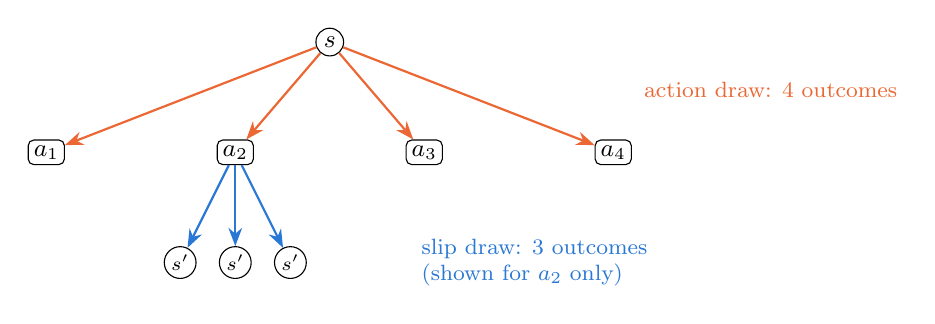
\begin{tikzpicture}[x=1cm,y=1cm,>=Stealth, every node/.style={font=\small}]
  \node[draw, circle, inner sep=1.5pt] (s) at (0,0) {$s$};
  \foreach \i/\x in {1/-3.6,2/-1.2,3/1.2,4/3.6} {
    \node[draw, rectangle, rounded corners=2pt, inner sep=2pt] (a\i) at (\x,-1.4) {$a_\i$};
    \draw[->, sampc, thick] (s) -- (a\i);
  }
  \node[sampc, font=\footnotesize] at (5.6,-0.6) {action draw: 4 outcomes};
  \foreach \j/\dx/\lab in {1/-0.7/left,2/0/straight,3/0.7/right} {
    \node[draw, circle, inner sep=1pt, font=\scriptsize] (t\j) at ({-1.2+\dx},-2.8) {$s'$};
    \draw[->, enumc, thick] (a2) -- (t\j);
  }
  \node[enumc, font=\footnotesize, align=left] at (2.6,-2.8) {slip draw: 3 outcomes\\(shown for $a_2$ only)};
\end{tikzpicture}
\end{center}

A step therefore fans out into up to $4\times 3=12$ branches if both draws are enumerated. Over $n$ steps that is
$12^n$ paths, but most of them end in the same few states: \textbf{safe merging} joins branches whose futures are
identical and adds their weights, so the work is bounded by the number of distinct states rather than paths
(Section~\ref{sec:cost}).

\paragraph{The hybrid winner, in code.} The configuration this study recommends for FrozenLake prediction is one line:
\begin{lstlisting}
SelectionRule rule = SelectionRule.hybrid(
    Map.of("action",     SelectionRule.budget(9),       // sample the policy draw, budget allocation
           "transition", SelectionRule.exhaustive()),   // enumerate the slip
    SelectionRule.exhaustive());                        // any other draw
\end{lstlisting}

\paragraph{Why it matters for control.} So far the RL track \emph{evaluates} a fixed policy, so the action is a draw
like any other, and it can even be folded into one joint draw $P^\pi(s'\mid s)$. In control (the next phase) the agent
\emph{chooses} the action that maximizes value. The search tree then alternates two kinds of nodes: \textbf{max nodes}
(actions; every action must be looked at, so they are always enumerated, and they cannot be folded into the
environment's law) and \textbf{chance nodes} (the environment's draws, here the slip; these are averaged, and can be
enumerated or sampled). The question ``enumerate or sample?'' then applies to the chance nodes only. This study answers
it for the slip: it is the noisy draw, its outcome set is small, and sampling it is the costliest way to lose precision.
The structure that control forces, ``enumerate action, sample slip'', is the worst of the sampled configurations
measured here, so a control search on FrozenLake should enumerate the slip as well and rely on merging.

%=====================================================================
\section{Setup}\label{sec:setup}

\takeaway{Every estimator computes the same $n$-step target, whose exact value is $V^\pi(s)$. We measure its bias,
its variance over independent seeds, its work in engine departures, and their product variance$\times$work, which
ranks unbiased estimators at equal compute.}

\paragraph{Target.} $\mathrm{target}(s)=E\big[\sum_{i=1}^{n}\gamma^{i-1}R_i+\gamma^nV(S_n)\mid S_0=s\big]$ with
$V(S_n)=0$ if the walk ends in a terminal state first. With $V=V^\pi$ the exact target equals $V^\pi(s)$ for every $n$
(Bellman consistency), so bias is measured against a known value. Policy: $\varepsilon$-soft greedy for $V^*$,
$\varepsilon=0.2$, $\gamma=0.99$ on FrozenLake; the random walk has one action and $\gamma=1$.

\paragraph{Measures.} For each start state: the mean, the variance over replications, and the mean work. Work is the
engine's departure count (model transitions run, including replays), the same unit for every method. For an unbiased
estimator the variance falls as $1/\text{work}$ when work is spent on replications, so
\[
\text{efficiency} = \text{variance}\times\text{work}
\qquad\text{and}\qquad
\text{work needed for a target s.d. }\sigma \;=\; \frac{\text{variance}\times\text{work}}{\sigma^2}.
\]
Lower efficiency is better. Tables report averages over start states: FrozenLake $\{0,10,18,33,44,57\}$, random walk
$\{4,7,10,13,16\}$.

\paragraph{Part A (hybrid selection).} FrozenLake in two-draw mode; $n\in\{2,4,6\}$; $k\in\{2,3\}$; budget $B=k^2$.
Per draw: enumerate, sample $k$, or budget; with and without safe merging. References: the one-joint-draw $k$-tree and
budget (the Compare\-NStep methods) and plain rollouts $N=k^2$. Up to 200 replications per start state, at least 30;
unmerged configurations whose live set exceeds 30k branches, or whose runs exceed 25k departures, are reported as
\emph{cap} or \emph{cost} instead of being replicated.

\paragraph{Part B (cost growth).} Both problems, one joint draw per step, $n=2,\dots,12$: exhaustive without merging
(live-set cap 50k), exhaustive with safe merging, $k$-trees $k=2,3$, budget $B=4,9$, and 9 rollouts, plus the
two-draw exhaustive expansion and the Part~A winner on FrozenLake, and the lag-free observation of
Section~\ref{sec:lag}. Sampled methods: 100 replications per start state (at least 35 for the costliest).

%=====================================================================
\section{Results A: which draw to enumerate}\label{sec:hybrid}

\takeaway{Enumerating the slip and sampling the action wins at every $n$ and $k$; with budget allocation for the
action it is the best of all sampled methods, $1.3$--$2.9\times$ better than the best one-draw sampler and
$2.3$--$6.7\times$ better than rollouts. Enumerating the action and sampling the slip is the worst merged choice.
Merging helps every configuration (up to $8\times$ for the same rule), and budget beats a fixed $k$. All estimators are
unbiased.}

\begin{table}[htbp]
\centering\footnotesize
% generated by rl/experiments/plot_hybrid_cost.py; do not edit
\begin{tabular}{@{}llrrrrrr@{}}
\toprule
 & & \multicolumn{3}{c}{$k=2$ ($B=4$)} & \multicolumn{3}{c}{$k=3$ ($B=9$)}\\
\cmidrule(lr){3-5}\cmidrule(l){6-8}
\textbf{Per-draw rule} & \textbf{Merge} & $n{=}2$ & $n{=}4$ & $n{=}6$ & $n{=}2$ & $n{=}4$ & $n{=}6$\\
\midrule
sample action ($k$), enumerate slip & none & $5.0{\times}10^{-3}$ & 0.18 & cost & $7.4{\times}10^{-3}$ & 0.61 & cap\\
sample action ($k$), enumerate slip & safe & $2.8{\times}10^{-3}$ & 0.021 & 0.080 & $2.7{\times}10^{-3}$ & 0.024 & 0.074\\
enumerate action, sample slip ($k$) & none & 0.038 & 1.8 & cap & 0.048 & cost & cap\\
enumerate action, sample slip ($k$) & safe & 0.017 & 0.17 & 0.57 & 0.015 & 0.12 & 0.54\\
sample both ($k$-tree) & none & 0.014 & 0.21 & 2.8 & 0.026 & 1.9 & cap\\
sample both ($k$-tree) & safe & $9.6{\times}10^{-3}$ & 0.054 & 0.20 & $8.3{\times}10^{-3}$ & 0.074 & 0.24\\
budget action ($B{=}k^2$), enumerate slip & safe & \textbf{\boldmath $2.2{\times}10^{-3}$} & \textbf{\boldmath 0.011} & \textbf{\boldmath 0.036} & \textbf{\boldmath $1.6{\times}10^{-3}$} & \textbf{\boldmath $8.0{\times}10^{-3}$} & \textbf{\boldmath 0.024}\\
enumerate action, budget slip ($B{=}k^2$) & safe & 0.010 & 0.12 & 0.44 & $6.9{\times}10^{-3}$ & 0.060 & 0.21\\
budget both ($B{=}k^2$) & safe & $8.3{\times}10^{-3}$ & 0.036 & 0.070 & $6.9{\times}10^{-3}$ & 0.031 & 0.061\\
one joint draw, $k$-tree & safe & $7.4{\times}10^{-3}$ & 0.030 & 0.080 & $7.1{\times}10^{-3}$ & 0.036 & 0.11\\
one joint draw, budget $B{=}k^2$ & safe & $4.9{\times}10^{-3}$ & 0.024 & 0.047 & $4.8{\times}10^{-3}$ & 0.020 & 0.042\\
plain rollouts, $N{=}k^2$ & none & 0.012 & 0.038 & 0.083 & 0.011 & 0.041 & 0.099\\
\bottomrule
\end{tabular}

\caption{Variance$\times$work (lower is better) of every sampled configuration, FrozenLake, two draws per step,
averaged over 6 start states. Bold: best in the column. \emph{cap}: the unmerged live set exceeded 30k branches;
\emph{cost}: more than 25k departures per run, not replicated.}
\label{tab:eff}
\end{table}

\begin{figure}[htbp]
\centering
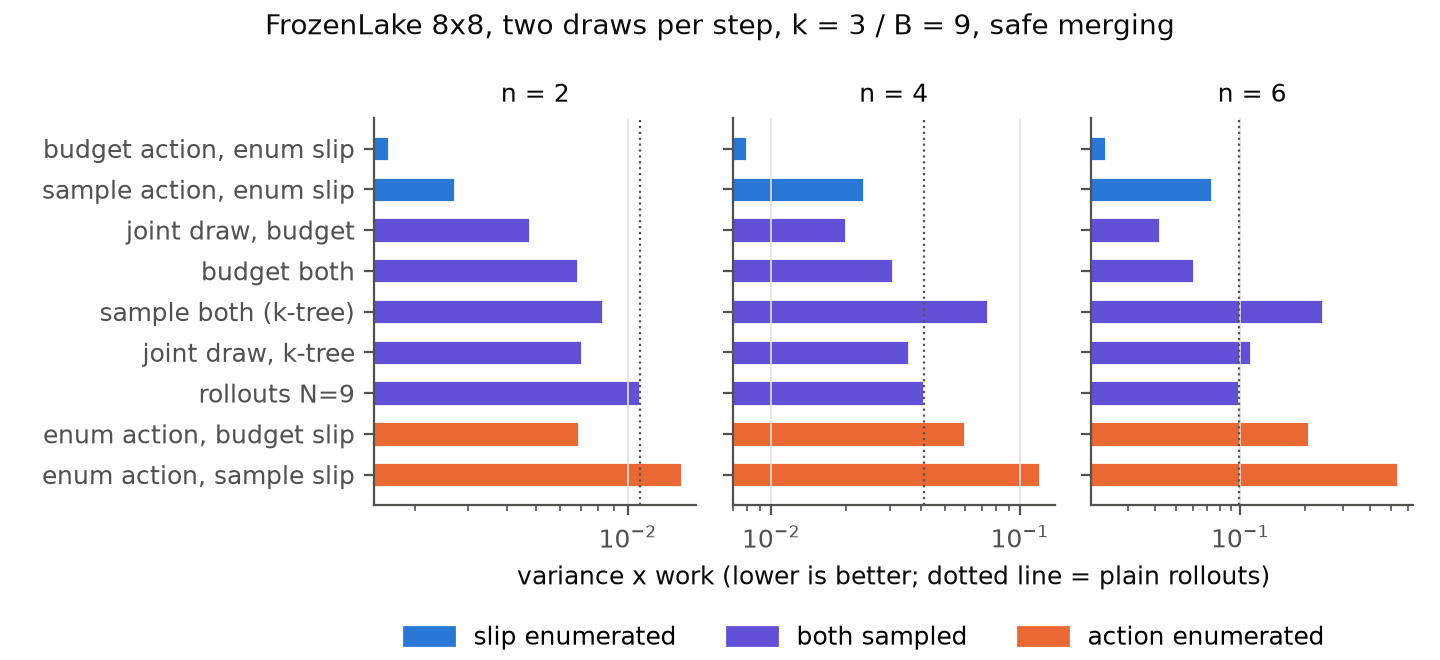
\includegraphics[width=\linewidth]{hybrid_efficiency.png}
\caption{Variance$\times$work at $k=3$ / $B=9$ with safe merging (log scale). Blue: slip enumerated; violet: both
sampled; orange: action enumerated. Dotted line: plain rollouts at the same sampling.}
\label{fig:eff}
\end{figure}

\paragraph{What the numbers say.}
\begin{enumerate}
\item \textbf{Enumerate the slip.} At $k=3$ with merging, ``sample action, enumerate slip'' beats ``enumerate action,
  sample slip'' by $5.5\times$ ($n=2$), $5.1\times$ ($n=4$) and $7.4\times$ ($n=6$) ($6$--$8\times$ at $k=2$), and with
  budget allocation the gap is $4$--$12\times$. Enumerating the slip costs about as much work as enumerating the action,
  but removes far more variance (Section~\ref{sec:split}).
\item \textbf{Budget beats fixed $k$.} With the slip enumerated, budget allocation for the action is $1.3$--$3.1\times$
  better than $k$ samples per action draw: merged branches get samples in proportion to their weight instead of $k$
  each.
\item \textbf{The best hybrid beats the joint draw.} One joint draw $P^\pi(s'\mid s)$ with budget is the best
  non-hybrid sampler ($4.8\times10^{-3}$, $0.020$, $0.042$ at $k=3$), and the hybrid improves on it by $2.9\times$,
  $2.5\times$, $1.8\times$ at $n=2,4,6$ ($2.2$, $2.2$, $1.3\times$ at $k=2$). The advantage shrinks with $n$ because the
  enumerated slip makes the merged live set grow faster (work 85 $\to$ 614).
\item \textbf{Merging always helps.} The same rule without merging is $1.8\times$ ($n=2$) to $8\times$ ($n=4$) worse and
  exceeds the caps by $n=6$.
\item \textbf{Exact is affordable here.} Enumerating both draws with merging costs 84, 664 and 2{,}240 departures at
  $n=2,4,6$. Against the best hybrid this is the cheaper option whenever the required s.d.\ is below
  $\sqrt{\text{eff}/W}=0.0044$, $0.0035$, $0.0033$; Section~\ref{sec:crossover} studies this crossover in detail.
\end{enumerate}

\begin{table}[htbp]
\centering\footnotesize
% generated by rl/experiments/plot_hybrid_cost.py; do not edit
\begin{tabular}{@{}lrrrrrr@{}}
\toprule
\textbf{Per-draw rule (safe merge)} & $n$ & $|$bias$|$ & max $|z|$ & variance & work & var$\times$work\\
\midrule
enumerate both (exact) & 2 & $1.3{\times}10^{-13}$ & -- & 0 & 84 & 0\\
sample action ($k$){,} enumerate slip & 2 & $3.5{\times}10^{-4}$ & 2.1 & $4.3{\times}10^{-5}$ & 61 & $2.7{\times}10^{-3}$\\
enumerate action{,} sample slip ($k$) & 2 & $8.5{\times}10^{-4}$ & 2.2 & $1.9{\times}10^{-4}$ & 83 & 0.015\\
sample both ($k$-tree) & 2 & $2.3{\times}10^{-4}$ & 1.6 & $1.4{\times}10^{-4}$ & 60 & $8.3{\times}10^{-3}$\\
budget action ($B{=}k^2$){,} enumerate slip & 2 & $3.0{\times}10^{-4}$ & 2.1 & $1.9{\times}10^{-5}$ & 85 & $1.6{\times}10^{-3}$\\
enumerate action{,} budget slip ($B{=}k^2$) & 2 & $3.4{\times}10^{-4}$ & 1.1 & $1.2{\times}10^{-4}$ & 58 & $6.9{\times}10^{-3}$\\
budget both ($B{=}k^2$) & 2 & $1.0{\times}10^{-3}$ & 2.0 & $1.5{\times}10^{-4}$ & 46 & $6.9{\times}10^{-3}$\\
one joint draw{,} $k$-tree & 2 & $5.0{\times}10^{-4}$ & 1.0 & $3.9{\times}10^{-4}$ & 18 & $7.1{\times}10^{-3}$\\
one joint draw{,} budget $B{=}k^2$ & 2 & $7.1{\times}10^{-4}$ & 1.2 & $1.7{\times}10^{-4}$ & 28 & $4.8{\times}10^{-3}$\\
plain rollouts{,} $N{=}k^2$ & 2 & $3.1{\times}10^{-4}$ & 1.2 & $1.6{\times}10^{-4}$ & 71 & 0.011\\
\midrule
enumerate both (exact) & 4 & $2.4{\times}10^{-13}$ & -- & 0 & 664 & 0\\
sample action ($k$){,} enumerate slip & 4 & $6.6{\times}10^{-4}$ & 2.5 & $5.0{\times}10^{-5}$ & 437 & 0.024\\
enumerate action{,} sample slip ($k$) & 4 & $1.0{\times}10^{-3}$ & 1.8 & $2.1{\times}10^{-4}$ & 646 & 0.12\\
sample both ($k$-tree) & 4 & $3.6{\times}10^{-4}$ & 1.3 & $1.8{\times}10^{-4}$ & 401 & 0.074\\
budget action ($B{=}k^2$){,} enumerate slip & 4 & $1.7{\times}10^{-4}$ & 1.3 & $3.2{\times}10^{-5}$ & 241 & $8.0{\times}10^{-3}$\\
enumerate action{,} budget slip ($B{=}k^2$) & 4 & $7.2{\times}10^{-4}$ & 1.9 & $2.3{\times}10^{-4}$ & 293 & 0.060\\
budget both ($B{=}k^2$) & 4 & $1.0{\times}10^{-3}$ & 1.7 & $3.5{\times}10^{-4}$ & 92 & 0.031\\
one joint draw{,} $k$-tree & 4 & $1.4{\times}10^{-3}$ & 3.1 & $5.0{\times}10^{-4}$ & 73 & 0.036\\
one joint draw{,} budget $B{=}k^2$ & 4 & $1.3{\times}10^{-3}$ & 2.4 & $3.6{\times}10^{-4}$ & 57 & 0.020\\
plain rollouts{,} $N{=}k^2$ & 4 & $6.4{\times}10^{-4}$ & 0.9 & $3.6{\times}10^{-4}$ & 120 & 0.041\\
\midrule
enumerate both (exact) & 6 & $3.5{\times}10^{-13}$ & -- & 0 & 2{,}240 & 0\\
sample action ($k$){,} enumerate slip & 6 & $3.6{\times}10^{-4}$ & 2.3 & $4.5{\times}10^{-5}$ & 1{,}466 & 0.074\\
enumerate action{,} sample slip ($k$) & 6 & $5.3{\times}10^{-4}$ & 0.7 & $2.8{\times}10^{-4}$ & 2{,}176 & 0.54\\
sample both ($k$-tree) & 6 & $9.6{\times}10^{-4}$ & 2.2 & $1.8{\times}10^{-4}$ & 1{,}343 & 0.24\\
budget action ($B{=}k^2$){,} enumerate slip & 6 & $4.2{\times}10^{-4}$ & 1.6 & $3.7{\times}10^{-5}$ & 614 & 0.024\\
enumerate action{,} budget slip ($B{=}k^2$) & 6 & $1.7{\times}10^{-3}$ & 2.1 & $2.9{\times}10^{-4}$ & 878 & 0.21\\
budget both ($B{=}k^2$) & 6 & $1.0{\times}10^{-3}$ & 1.3 & $4.9{\times}10^{-4}$ & 134 & 0.061\\
one joint draw{,} $k$-tree & 6 & $1.2{\times}10^{-3}$ & 1.8 & $5.6{\times}10^{-4}$ & 212 & 0.11\\
one joint draw{,} budget $B{=}k^2$ & 6 & $1.3{\times}10^{-3}$ & 2.4 & $5.3{\times}10^{-4}$ & 86 & 0.042\\
plain rollouts{,} $N{=}k^2$ & 6 & $1.8{\times}10^{-3}$ & 2.8 & $6.7{\times}10^{-4}$ & 163 & 0.099\\
\bottomrule
\end{tabular}

\caption{Detail at $k=3$, $B=9$ with safe merging (rollouts: no merging), averaged over 6 start states.
max $|z|$: largest $|\text{mean}-\text{exact}|/\text{s.e.}$ over the start states.}
\label{tab:detail}
\end{table}

\paragraph{Bias.} Over the 396 (configuration, start state) cells of Part~A the largest $|z|$ is 3.1 and most are below
2 (Part~B: about 800 cells, largest 3.15), as expected of unbiased estimators tested this many times. Exact configurations match $V^\pi(s)$ to $10^{-13}$.
\code{VerifyHybrid} adds four 4-standard-error checks on the hybrids and runs in the default build.

%=====================================================================
\section{Where the variance comes from}\label{sec:split}

\takeaway{The law of total variance splits the variance of one rollout's target exactly into a policy part and a slip
part. The slip carries 88\% of it (77--95\% depending on the start state), so it is the draw worth enumerating; the
split matches the observed rollout variance. The ``enumerate the noisiest small draw'' rule is therefore grounded: rank
draws by variance share per outcome.}

\paragraph{The decomposition.} With $V=V^\pi$ the rollout target is a sum of martingale increments,
\[
G = V(s_0) + \sum_{t=0}^{n-1}\gamma^t D_t,\qquad D_t = R_{t+1}+\gamma V(S_{t+1})-V(S_t),\qquad E[D_t\mid S_t]=0,
\]
so the increments are uncorrelated and $\operatorname{Var}G=\sum_t\gamma^{2t}E\big[\operatorname{Var}(Y_t\mid S_t)\big]$ with
$Y_t=R_{t+1}+\gamma V(S_{t+1})$. Within a step, conditioning on the action $A$ (law of total variance):
\[
\operatorname{Var}(Y\mid s) \;=\; \underbrace{\operatorname{Var}_A\big(E[Y\mid s,A]\big)}_{\text{policy part}}
\;+\; \underbrace{E_A\big[\operatorname{Var}(Y\mid s,A)\big]}_{\text{slip part}} .
\]
Both parts are computed exactly from the tables, with the exact distribution of $S_t$ (no sampling), in
\code{CompareHybrid.split}.

\begin{table}[htbp]
\centering\footnotesize
% generated by rl/experiments/plot_hybrid_cost.py; do not edit
\begin{tabular}{@{}rrrrrr@{}}
\toprule
$n$ & \textbf{Start} & \textbf{Policy part} & \textbf{Slip part} & \textbf{Policy share} & \textbf{Observed rollout var.}\\
\midrule
1 & 0 & $4.6{\times}10^{-7}$ & $7.4{\times}10^{-6}$ & 6\% & $7.8{\times}10^{-6}$ $\pm$ $2{\times}10^{-7}$\\
1 & 10 & $2.7{\times}10^{-5}$ & $1.2{\times}10^{-4}$ & 19\% & $1.4{\times}10^{-4}$ $\pm$ $3{\times}10^{-6}$\\
1 & 18 & $2.9{\times}10^{-4}$ & $1.4{\times}10^{-3}$ & 17\% & $1.6{\times}10^{-3}$ $\pm$ $4{\times}10^{-5}$\\
1 & 33 & $1.4{\times}10^{-4}$ & $9.2{\times}10^{-4}$ & 13\% & $1.1{\times}10^{-3}$ $\pm$ $2{\times}10^{-5}$\\
1 & 44 & $1.3{\times}10^{-4}$ & $1.7{\times}10^{-3}$ & 7\% & $1.9{\times}10^{-3}$ $\pm$ $4{\times}10^{-5}$\\
1 & 57 & $1.9{\times}10^{-5}$ & $1.9{\times}10^{-4}$ & 9\% & $2.1{\times}10^{-4}$ $\pm$ $5{\times}10^{-6}$\\
\multicolumn{2}{l}{mean, $n=1$} & $1.0{\times}10^{-4}$ & $7.2{\times}10^{-4}$ & 12\% & \\
\midrule
6 & 0 & $5.5{\times}10^{-5}$ & $3.4{\times}10^{-4}$ & 14\% & $3.8{\times}10^{-4}$ $\pm$ $8{\times}10^{-6}$\\
6 & 10 & $4.6{\times}10^{-4}$ & $1.9{\times}10^{-3}$ & 19\% & $2.4{\times}10^{-3}$ $\pm$ $5{\times}10^{-5}$\\
6 & 18 & $5.8{\times}10^{-4}$ & $3.5{\times}10^{-3}$ & 14\% & $4.0{\times}10^{-3}$ $\pm$ $9{\times}10^{-5}$\\
6 & 33 & $3.4{\times}10^{-4}$ & $3.5{\times}10^{-3}$ & 9\% & $3.9{\times}10^{-3}$ $\pm$ $9{\times}10^{-5}$\\
6 & 44 & $1.2{\times}10^{-3}$ & 0.016 & 7\% & 0.016 $\pm$ $4{\times}10^{-4}$\\
6 & 57 & $8.5{\times}10^{-5}$ & $6.7{\times}10^{-4}$ & 11\% & $7.7{\times}10^{-4}$ $\pm$ $2{\times}10^{-5}$\\
\multicolumn{2}{l}{mean, $n=6$} & $4.5{\times}10^{-4}$ & $4.3{\times}10^{-3}$ & 9\% & \\
\bottomrule
\end{tabular}

\caption{Exact split of one rollout's variance, FrozenLake. Observed: 4{,}000 rollouts per cell, $\pm$ one standard
error under a normal approximation (the returns are heavy-tailed, so this under-states the true error).}
\label{tab:split}
\end{table}

\begin{figure}[htbp]
\centering
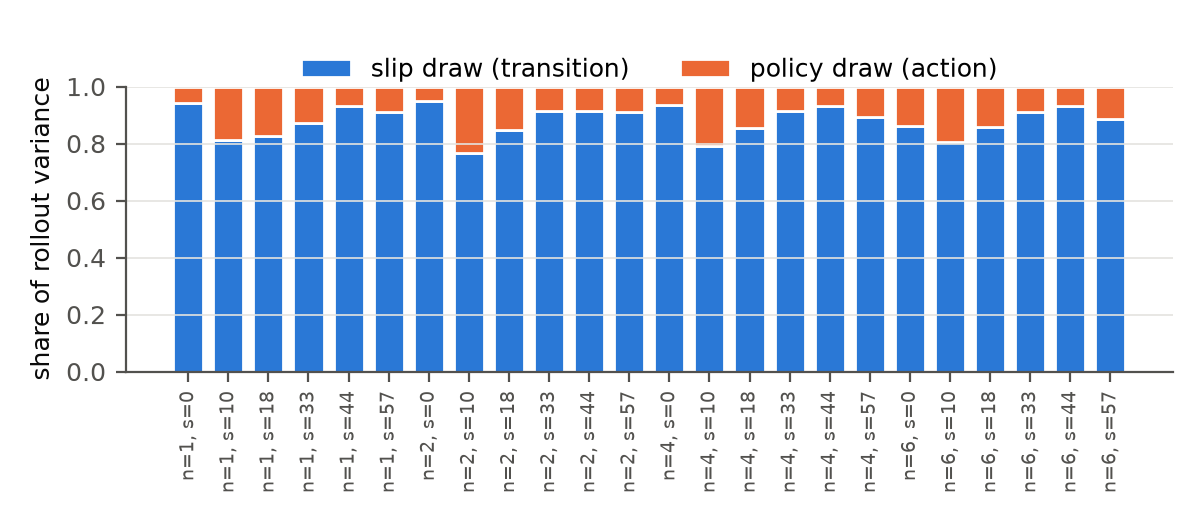
\includegraphics[width=0.85\linewidth]{hybrid_variance_split.png}
\caption{Share of the rollout variance due to each draw, for every start state and $n=1,2,4,6$.}
\label{fig:split}
\end{figure}

\paragraph{Why the slip dominates.} The $\varepsilon$-soft policy takes the greedy action with probability 0.85, and
the actions it mixes in lead to similar values; the ice moves the agent sideways two times out of three whatever it
chooses. The policy share is largest (19--23\%) at state 10, where the greedy action matters most.

\paragraph{The grounded rule.} Enumerating a draw with $b_d$ outcomes multiplies the work at that draw by about $b_d$
(instead of $k$) and removes its share $v_d$ of the variance. Rank the draws by $v_d/b_d$ and enumerate from the top:
slip $0.88/3=0.29$, action $0.12/4=0.03$. The measured efficiencies agree: the slip-enumerated configurations are
$4$--$12\times$ better than the action-enumerated ones (Table~\ref{tab:eff}).

%=====================================================================
\section{Results B: how the cost grows with \texorpdfstring{$n$}{n}}\label{sec:cost}

\takeaway{Without merging, exact work grows exponentially ($\times3.6$ per step on FrozenLake) and passes the cap at
$n=9$. With safe merging it is bounded by the reachable states: it grows while the set of live states fills up, then
linearly, from $n\approx11$ on FrozenLake and $n\approx14$ on the random walk. Sampled methods grow linearly from the
start, the budget ones slowest.}

\begin{table}[htbp]
\centering\footnotesize
% generated by rl/experiments/plot_hybrid_cost.py; do not edit
\begin{tabular}{@{}lrrrrrr@{}}
\toprule
\textbf{Method} & $n{=}2$ & $n{=}4$ & $n{=}6$ & $n{=}8$ & $n{=}10$ & $n{=}12$\\
\midrule
\multicolumn{7}{@{}l}{\textit{FrozenLake 8x8}: work per target}\\
exhaustive, no merge & 34 & 407 & 5{,}060 & 66{,}232 & cap & cap\\
exhaustive + merge & 34 & 229 & 730 & 1{,}637 & 2{,}954 & 4{,}609\\
exhaustive + merge, lag-free key & 30 & 128 & 332 & 665 & 1{,}115 & 1{,}642\\
exhaustive + merge, two draws & 84 & 664 & 2{,}240 & 5{,}154 & 9{,}441 & 14{,}891\\
$k$-tree $k{=}2$ + merge & 12 & 34 & 80 & 173 & 315 & 529\\
$k$-tree $k{=}3$ + merge & 18 & 73 & 208 & 484 & 925 & 1{,}575\\
budget $B{=}4$ + merge & 16 & 29 & 42 & 54 & 66 & 77\\
budget $B{=}9$ + merge & 28 & 58 & 85 & 113 & 137 & 161\\
budget $B{=}9$ + merge, lag-free key & 28 & 54 & 80 & 104 & 128 & 151\\
rollouts $N{=}9$ & 53 & 86 & 115 & 143 & 170 & 195\\
hybrid: budget action, enum slip & 85 & 242 & 614 & 1{,}290 & 2{,}306 & 3{,}669\\
\midrule
\multicolumn{7}{@{}l}{\textit{random walk 19}: work per target}\\
exhaustive, no merge & 14 & 62 & 249 & 977 & 3{,}808 & 14{,}816\\
exhaustive + merge & 14 & 48 & 102 & 174 & 260 & 356\\
exhaustive + merge, lag-free key & 13 & 36 & 69 & 110 & 158 & 211\\
$k$-tree $k{=}2$ + merge & 11 & 28 & 56 & 94 & 139 & 190\\
$k$-tree $k{=}3$ + merge & 15 & 48 & 102 & 173 & 266 & 373\\
budget $B{=}4$ + merge & 15 & 29 & 43 & 57 & 70 & 84\\
budget $B{=}9$ + merge & 26 & 54 & 82 & 110 & 139 & 166\\
budget $B{=}9$ + merge, lag-free key & 25 & 50 & 76 & 101 & 127 & 152\\
rollouts $N{=}9$ & 54 & 90 & 125 & 159 & 193 & 225\\
\bottomrule
\end{tabular}

\caption{Work per target (departures), averaged over start states. Sampled rows: mean work of one run.
\emph{cap}: the unmerged live set exceeded 50k branches.}
\label{tab:cost}
\end{table}

\begin{figure}[htbp]
\centering
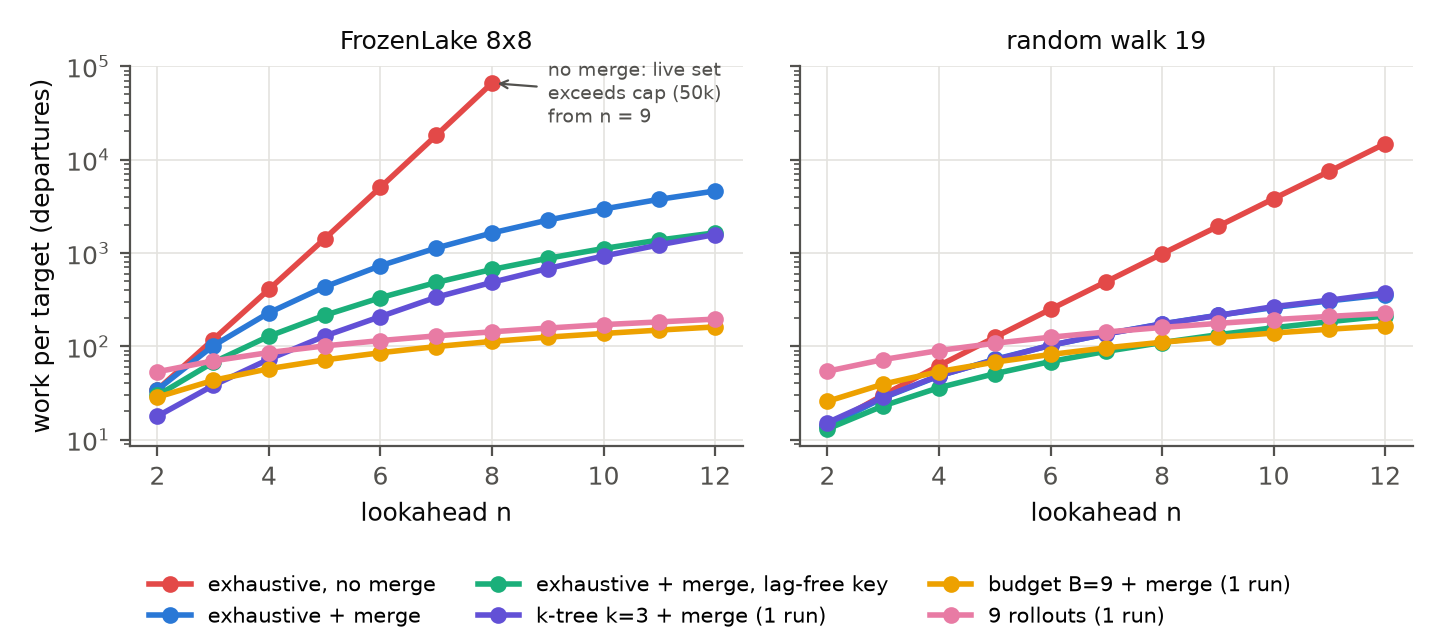
\includegraphics[width=\linewidth]{cost_growth.png}
\caption{Work per target against the lookahead $n$ (log scale).}
\label{fig:cost}
\end{figure}

\paragraph{Without merging.} FrozenLake's one-draw step has 3 or 4 distinct successors, so the tree grows by
$\times3.6$ per step: 407 departures at $n=4$, 5{,}060 at $n=6$, 66{,}232 at $n=8$, and the live set passes the 50k cap
at $n=9$. The random walk doubles per step (14{,}816 at $n=12$).

\paragraph{With merging: saturation.} Merged branches are distinct states, so the work of one more step is the cost of
expanding the live states: $1+b(s)$ departures for a state with $b(s)$ outcomes (one run that stops at the draw plus one
per outcome). Once every reachable state is live, this cost stops growing and the total becomes linear in $n$
(Figure~\ref{fig:sat}). FrozenLake has $|R|=53$ reachable live states with $\sum_{s\in R}(1+b(s))=262$ (mean branching
3.9); the live set is complete from $n\approx11$, after which each step adds about 272 departures (262 plus the
reports of walks ending in holes or the goal). The random walk has 19 states but, by parity, only about half of them are
live at any step, so each step adds about 30 departures from $n\approx14$, below the bound $\sum(1+b)=57$. Hence
\[
W_{\text{exact}}(n)\;\approx\;\sum_{t<n}|L_t|\,(1+b)\;\le\; n\,|R|\,(1+b),
\]
linear once saturated, against $b^n$ without merging.

\subsection{A finding: the observation lags the state}\label{sec:lag}

\takeaway{Safe merging keys a branch by its model state \emph{and} its observation. \code{MdpWalker} reports a state
one event after reaching it, so at the moment the engine merges, the observation still holds the previous state, and
branches merge only on (previous state, state) pairs. Keeping the state out of the observation (\code{LagFreeWalker})
merges on the state alone: the same exact targets for up to $2.8\times$ less work. Both work counts are predicted
exactly by counting reachable states and pairs.}

A DEVS model emits its output \emph{before} its internal transition (the eager $\psi\lambda$ convention). In
\code{MdpWalker}, event $k$ reports the current state and then draws the next one; the new state is reported at
event $k+1$. The engine merges right after a draw, when the transducer's observation $\xi$ (return, \emph{last
reported state}, steps) still holds the parent's state. Two branches that reach the same state from different parents
have different $\xi$, so they are merged only one step later, after they have each been expanded once. The live nodes
are therefore the reachable \emph{edges} (209 on FrozenLake, 38 on the random walk), not the states (53 and 19).

\code{LagFreeWalker} (new, in \code{examples.rl}) keeps the model and changes only what is observed: $\xi$ holds the
return and the step count; the model flags its final report on a second port, and the transducer adds the bootstrap
term $\gamma^nV(S_n)$ there. Nothing about the state remains in $\xi$, so branches merge on the state. The targets are
identical (checked to $10^{-12}$). The work drops from 4{,}609 to 1{,}642 departures on FrozenLake at $n=12$ and from
356 to 211 on the random walk, and the per-step cost at saturation from about 895 to 272 (FrozenLake). The two
level-by-level formulas in \code{CostGrowth.reach} reproduce the engine's departure counts exactly at every measured
$n$ (crosses in Figure~\ref{fig:sat}), and \code{VerifyHybrid} checks both.

\begin{figure}[htbp]
\centering
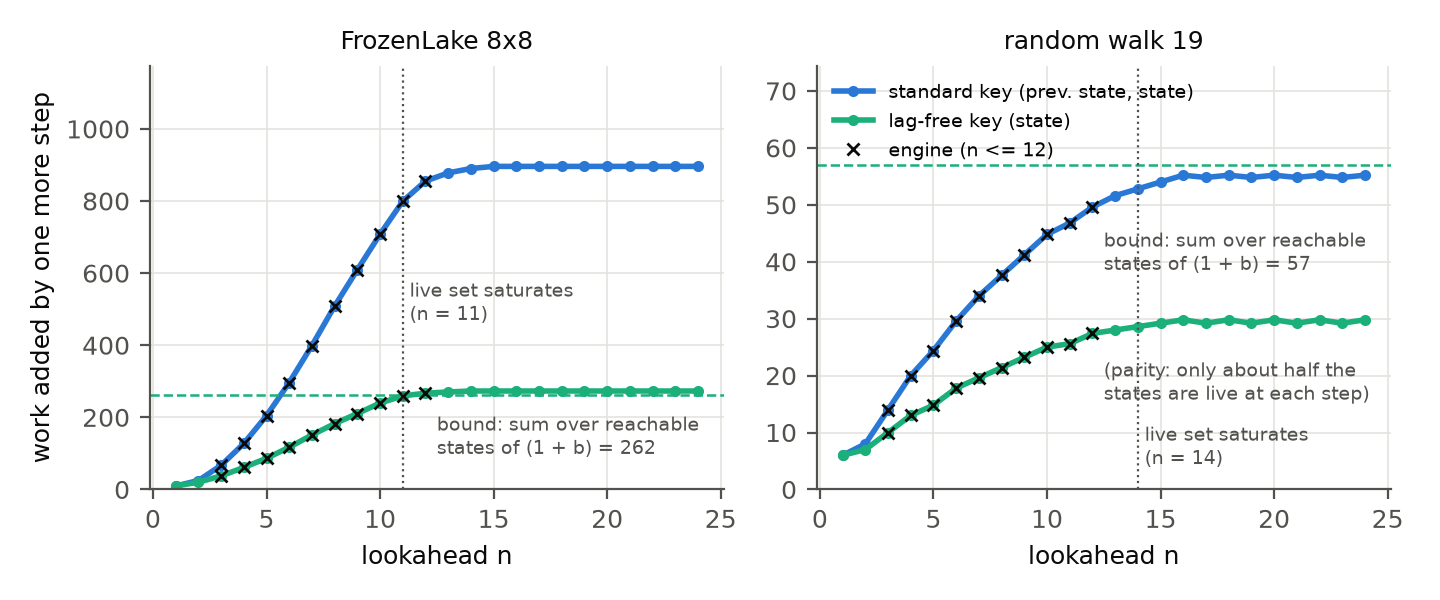
\includegraphics[width=\linewidth]{cost_saturation.png}
\caption{Work added by one more step of exact merged expansion. Lines: the level-by-level prediction (to $n=24$);
crosses: the engine ($n\le12$). The dashed line is the bound $\sum_{s\in R}(1+b(s))$; the dotted line marks where the
live set is complete.}
\label{fig:sat}
\end{figure}

\note{The lag is a property of the transducer, not of the engine: the engine merges exactly as specified (equal model
state and equal observation). The lesson for model authors is to keep the observation lean, recording only what the
query needs. Part~A used the standard \code{MdpWalker}, so all its configurations share the lag and their ranking is
unaffected; its exact rows would be cheaper with the lag-free observation.}

%=====================================================================
\section{The crossover: when exact expansion is cheaper}\label{sec:crossover}

\takeaway{For each $n$, exact merged expansion is cheaper than the best sampler whenever the required standard deviation
of the target is below $\sigma^*=\sqrt{\text{eff}_{\text{best}}/W_{\text{exact}}}$. $\sigma^*$ hardly depends on $n$:
0.005--0.007 on FrozenLake (0.007--0.010 lag-free) and 0.06--0.08 on the random walk (0.07--0.10). In rollout units
(lag-free, $n\ge4$): exact wins once you would need more than about 60--115 (FrozenLake) or 7--15 (random walk)
rollouts.}

\paragraph{Definition.} A sampled method with efficiency $\text{eff}=\text{variance}\times\text{work}$ needs work
$\text{eff}/\sigma^2$ to reach s.d.\ $\sigma$. Exact merged expansion costs $W_{\text{exact}}$ once, with s.d.\ 0. Exact is
cheaper when
\[
\sigma \;<\; \sigma^* \;=\; \sqrt{\text{eff}_{\text{best}}/W_{\text{exact}}},
\]
with $\text{eff}_{\text{best}}$ the best sampled method at that $n$. Expressed as a number of independent rollouts (each
of variance $\sigma_1^2$), exact wins once the precision needed is worth more than
$N^*=W_{\text{exact}}\,\sigma_1^2/\text{eff}_{\text{best}}$ rollouts.

\begin{table}[htbp]
\centering\footnotesize
% generated by rl/experiments/plot_hybrid_cost.py; do not edit
\begin{tabular}{@{}rlrrrrrrr@{}}
\toprule
 & & & \multicolumn{2}{c}{\textbf{Exact work}} & \multicolumn{2}{c}{\textbf{Crossover s.d.\ $\sigma^*$}} & \multicolumn{2}{c}{\textbf{Rollouts equiv.}}\\
\cmidrule(lr){4-5}\cmidrule(lr){6-7}\cmidrule(l){8-9}
$n$ & \textbf{Best sampled} & \textbf{var$\times$work} & std & lag-free & std & lag-free & std & lag-free\\
\midrule
\multicolumn{9}{@{}l}{\textit{FrozenLake 8x8}}\\
2 & hybrid (enum slip) & $1.6{\times}10^{-3}$ & 34 & 30 & 0.0067 & 0.0073 & 30 & 26\\
4 & hybrid (enum slip) & $6.6{\times}10^{-3}$ & 229 & 128 & 0.0054 & 0.0072 & 118 & 66\\
6 & hybrid (enum slip) & 0.021 & 730 & 332 & 0.0054 & 0.0080 & 137 & 62\\
8 & hybrid (enum slip) & 0.048 & 1{,}637 & 665 & 0.0054 & 0.0085 & 159 & 65\\
10 & budget $B{=}9$ & 0.096 & 2{,}954 & 1{,}115 & 0.0057 & 0.0093 & 229 & 86\\
12 & budget $B{=}9$ & 0.13 & 4{,}609 & 1{,}642 & 0.0052 & 0.0088 & 274 & 97\\
\midrule
\multicolumn{9}{@{}l}{\textit{random walk 19}}\\
2 & budget $B{=}9$ & 0.056 & 14 & 13 & 0.0632 & 0.0656 & 5 & 4\\
4 & budget $B{=}9$ & 0.22 & 48 & 36 & 0.0670 & 0.0773 & 10 & 7\\
6 & budget $B{=}9${,} lag-free & 0.45 & 102 & 69 & 0.0661 & 0.0806 & 13 & 9\\
8 & budget $B{=}9${,} lag-free & 0.90 & 174 & 110 & 0.0719 & 0.0904 & 14 & 9\\
10 & budget $B{=}9${,} lag-free & 1.4 & 260 & 158 & 0.0727 & 0.0933 & 17 & 10\\
12 & budget $B{=}9${,} lag-free & 1.8 & 356 & 211 & 0.0705 & 0.0916 & 25 & 15\\
\bottomrule
\end{tabular}

\caption{Crossover per $n$ (even $n$ shown; \texttt{cost\_crossover.csv} has all). Best sampled: lowest
variance$\times$work among the sampled methods of Part~B (FrozenLake includes the Part~A winner). Exact work with the
standard and the lag-free observation; $\sigma^*$ and the equivalent number of rollouts for each.}
\label{tab:cross}
\end{table}

\begin{figure}[htbp]
\centering
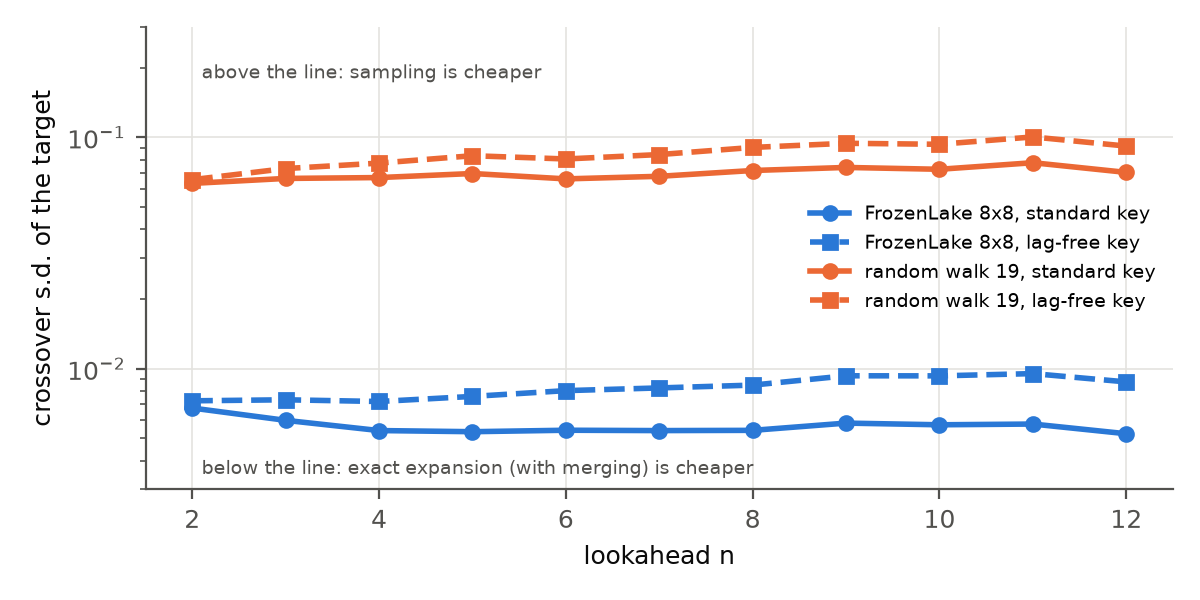
\includegraphics[width=0.85\linewidth]{cost_crossover.png}
\caption{Crossover standard deviation $\sigma^*$ against $n$. Below a line, exact merged expansion is cheaper than the
best sampler; above it, sampling is cheaper.}
\label{fig:cross}
\end{figure}

\paragraph{Why $\sigma^*$ is flat in $n$.} Both sides grow at about the same rate. The best sampler's efficiency grows
roughly like $n^2$ (variance $\propto n$ before termination, work $\propto n$), and exact merged work grows like
$\sum_t|L_t|$, which is superlinear while the live set fills and linear after. Their ratio drifts only slowly; on
FrozenLake the lag-free $\sigma^*$ rises from 0.0073 to 0.0088 between $n=2$ and $n=12$.

\paragraph{Scale.} The FrozenLake targets are of order 0.1 (e.g.\ $V^\pi(18)=0.132$), so $\sigma^*\approx0.005$--0.009 is a
relative precision of about 5\%: exact expansion is the cheaper choice for any learner that wants targets better than
that. On the random walk ($|V|\le1$) the crossover is at about 0.07--0.09.

%=====================================================================
\section{Rule of thumb}\label{sec:rule}

\takeaway{Enumerate everything (with merging) if the precision you need is worth more than about $|R|(1+b)/2$
rollouts; otherwise go hybrid, enumerating the small draws that carry most of the variance and sampling the rest with
budget allocation. Merge in every case.}

\paragraph{Derivation.} After saturation, exact merged work is at most $n\sum_{s\in R}(1+b(s))\approx n|R|(1+b)$
(lag-free observation; with the lagged one, replace $|R|$ by the number of reachable edges). A rollout costs about $2n$
departures (one run that stops at the draw and one that completes, per step). Exact therefore beats $N$ rollouts once
$N > |R|(1+b)/2$; better samplers move the crossover up by their gain $1/\rho$ ($\rho$ = their efficiency relative to
rollouts, 0.2--0.9 here). In terms of the target s.d.:
\[
\text{enumerate if}\quad \sigma \;<\; \sigma_1\sqrt{\frac{2}{|R|\,(1+b)}},
\]
with $\sigma_1$ the s.d.\ of one rollout's target (a pilot of about 100 rollouts estimates it). For FrozenLake
($|R|=53$, $\sum(1+b)=262$, $\sigma_1\approx0.04$--0.10 from $n=2$ to 12) this gives 0.003--0.009 against the
measured 0.007--0.010 (lag-free); for the random walk ($|R|=19$, $\sum(1+b)=57$) 0.025--0.066 against 0.066--0.100. The
rule is conservative: in this data it never recommends exact expansion where sampling would have been cheaper, because
the bound ignores parity and the unsaturated early levels (which make exact cheaper than the bound), and it compares
with plain rollouts (better samplers have $\rho<1$, which works the other way but is outweighed here).

\paragraph{The procedure.}
\begin{enumerate}
\item \textbf{Merge always}, and keep the observation lean (Section~\ref{sec:lag}).
\item \textbf{Count} the reachable live states $|R|$ within the horizon and the outcomes per step $b$ (product over the
  draws that would be enumerated).
\item \textbf{Exact if} the required s.d.\ is below $\sigma_1\sqrt{2/(|R|(1+b))}$, or you need distributions rather
  than means, or $|R|(1+b)$ is a few hundred or less (exact is then cheap in absolute terms: under 5k departures per
  target on FrozenLake at $n=12$).
\item \textbf{Otherwise hybrid}: for each draw estimate its variance share $v_d$ (law of total variance, as in
  Section~\ref{sec:split}) and its outcome count $b_d$; enumerate the draws with the largest $v_d/b_d$ while the merged
  work stays affordable; sample the rest with \code{budget(B)}, not a fixed $k$.
\item \textbf{Large or continuous draws} are always sampled; budget allocation with merging is the safe default.
\item \textbf{In control}: actions are max nodes and are always enumerated. Treat the environment's draws as chance
  nodes and apply steps 3--5 to them alone; for FrozenLake that means enumerating the slip, i.e.\ full enumeration with
  merging (2{,}240 departures at $n=6$ with the standard observation).
\end{enumerate}

%=====================================================================
\section{Caveats}\label{sec:caveats}

\takeaway{Two small tabular problems, one policy, $V=V^\pi$ bootstrapping, and rewards only on terminal arrival. The
qualitative conclusions should carry over; the constants will not.}

\begin{itemize}
\item \textbf{Merging is easy here.} Rewards arrive only on reaching a terminal state, so every live branch has return 0
  and merging depends on the state alone. With rewards on every step, safe merging also needs equal accumulated returns
  and fires far less (RL Plan, variance section); the expectation-only merge (opt-in, off by default) restores it for
  means only.
\item \textbf{Work is counted in departures}, the engine's unit. Wall-clock time also depends on snapshot size (about
  15k departures per second per thread on this machine) and on bookkeeping that grows with the live set.
\item \textbf{$V=V^\pi$} makes the exact answer known and the increments a martingale. With an approximate $V$, the
  target is biased by the bootstrap term identically for all methods, and the variance split gains cross terms.
\item \textbf{Replications.} 100--200 per start state (at least 30--35 for the costliest), so variances carry about
  10--25\% relative error; efficiency ratios below about $1.3\times$ are not significant. The returns are heavy-tailed
  (rare goal arrivals), which makes variance estimates noisier than the normal approximation suggests.
\item \textbf{The crossover uses averages over start states} of variance$\times$work; individual states differ by more than
  $10\times$ in variance (Table~\ref{tab:split}).
\item \textbf{Caps.} Unmerged configurations were capped at 30k (Part~A) or 50k (Part~B) live branches, so the
  exponential curves stop where the cap is reached.
\item \textbf{One policy.} With a greedier policy the policy share of the variance falls further; with a uniform policy it
  rises, and ``enumerate the action'' could become competitive. The ranking rule ($v_d/b_d$) covers both cases.
\item \textbf{Part~A used the lagged observation}; its exact and merged work would be lower with \code{LagFreeWalker}, which
  would move its crossover up, but not change which hybrid wins.
\end{itemize}

%=====================================================================
\section{Reproducing the study}\label{sec:repro}

\takeaway{Two Java drivers write resumable CSVs in chunks of under three minutes; a Python script makes the figures and
tables; a 12-check test runs in the default build.}

\begin{tabularx}{\linewidth}{@{}>{\raggedright\arraybackslash}p{5.6cm}Y@{}}
\toprule
\textbf{File} & \textbf{What it does}\\
\midrule
\path{examples/rl/CompareHybrid.java} & Part~A and the variance split; \path{hybrid_study.csv},
  \path{hybrid_variance_split.csv}\\
\path{examples/rl/CostGrowth.java} & Part~B and the reachable-set predictions; \path{cost_growth.csv},
  \path{cost_reach.csv}\\
\path{examples/rl/HybridRuns.java} & shared harness: per-draw rules, replicated runs on 3 threads, resumable CSV\\
\path{examples/rl/LagFreeWalker.java} & the walker with a lean observation (Section~\ref{sec:lag})\\
\path{examples/rl/VerifyHybrid.java} & 12 checks (build test \code{hybrid}, about 15\,s)\\
\path{rl/experiments/plot_hybrid_cost.py} & figures, \path{cost_crossover.csv}, and the \path{hybrid_tab_*.tex} tables\\
\bottomrule
\end{tabularx}

\begin{lstlisting}[language=bash]
JAVA_TOOL_OPTIONS=-Xmx512m bash scripts/build_library.sh hybrid       # build + checks
CP="build/library/classes;lib/ms4-core.jar"
java -Xmx512m -Dn=4 -Dbudget=170 -cp "$CP" examples.rl.CompareHybrid    # repeat until done
java -Xmx512m -Dproblem=fl -Dbudget=170 -cp "$CP" examples.rl.CostGrowth
rl/.venv/Scripts/python.exe rl/experiments/plot_hybrid_cost.py
\end{lstlisting}
Each driver stops after its time budget (\code{-Dbudget}, seconds) and skips rows already in its CSV when rerun. The
whole study took about 30 minutes of compute on one JVM (\code{-Xmx512m}, 3 worker threads), in chunks of under three
minutes.

%=====================================================================
\appendix
\section{Glossary}\label{app:glossary}

\begin{tabularx}{\linewidth}{@{}>{\bfseries\raggedright\arraybackslash}p{3.4cm}Y@{}}
\toprule
Draw & One random choice a model makes, \code{Para.choose(label, law)}; here ``action'' (the policy) and
  ``transition'' (the slip).\\
Outcome, branching $b$ & A possible value of a draw; $b$ is the number of outcomes per step.\\
Enumerate (exhaustive) & Follow every outcome, weighted by its probability: exact, no noise.\\
Sample ($k$) & Follow $k$ random outcomes, each with weight $1/k$: unbiased, noisy. A $k$-tree samples $k$ at every draw.\\
Budget allocation $B$ & A branch of weight $w$ draws $\max(1,\mathrm{round}(Bw))$ samples; with merging, about $B$ per level.\\
Hybrid selection & A selection rule per draw label (\code{SelectionRule.hybrid}).\\
Joint draw & The action and the slip folded into one draw from $P^\pi(s'\mid s)$; possible only for a fixed policy.\\
Safe merging & Joining branches with equal model state and equal observation, adding their weights; exact for any query.\\
Observation $\xi$ & What the transducer records from the model's outputs (here: return, steps, and in \code{MdpWalker}
  the last reported state). Part of the merge key.\\
Lag & In \code{MdpWalker}, $\xi$ holds the previous state at the moment of merging, so merges happen on (previous state,
  state) pairs.\\
Departure, work & One run of a model transition by the engine, including replays; the unit of work.\\
Efficiency & Variance$\times$work. Work needed for target s.d.\ $\sigma$ is efficiency$/\sigma^2$. Lower is better.\\
Bias, $z$ & Mean minus exact value; $z$ divides it by the standard error.\\
Live set $L_t$ & The distinct live (non-terminal) branches after $t$ steps.\\
Reachable set $R$ & The live states reachable within the horizon.\\
Saturation & The point where $L_t$ stops growing; merged exact work is linear in $n$ after it.\\
Crossover $\sigma^*$ & The target s.d.\ below which exact merged expansion is cheaper than the best sampler.\\
Law of total variance & $\operatorname{Var}Y=E[\operatorname{Var}(Y\mid A)]+\operatorname{Var}(E[Y\mid A])$; here it splits the
  variance into slip and policy parts.\\
Max node, chance node & In a control search: an action choice (maximized, always enumerated) and an environment draw
  (averaged; enumerated or sampled).\\
$n$-step target & $E[\sum_{i\le n}\gamma^{i-1}R_i+\gamma^nV(S_n)]$; with $V=V^\pi$ it equals $V^\pi(s)$.\\
$\varepsilon$-soft policy & Greedy action with probability $1-\varepsilon+\varepsilon/4$, each other action
  $\varepsilon/4$.\\
\bottomrule
\end{tabularx}

\end{document}
